Die bisherigen Szenarien nutzen eine statische Kamera. Das erlaubt zwar konstante Messungen, entspricht allerdings keiner realistischen Situation. Normalerweise wird die Kamera bewegt und rotiert. Die folgenden Szenarien stellen dynamische Situationen dar, in denen die Kamera bewegt wird. In diesem Szenario wird die Kamera dauerhaft rotiert mit einer Winkelgeschwindigkeit von \SI{45}{\degree\per\second}. Eine Reihe von Screenshots, die die Rotation zeigt, ist in Abbildung~\vref{fig:rotate} zu sehen.
\begin{figure}
	\centering
	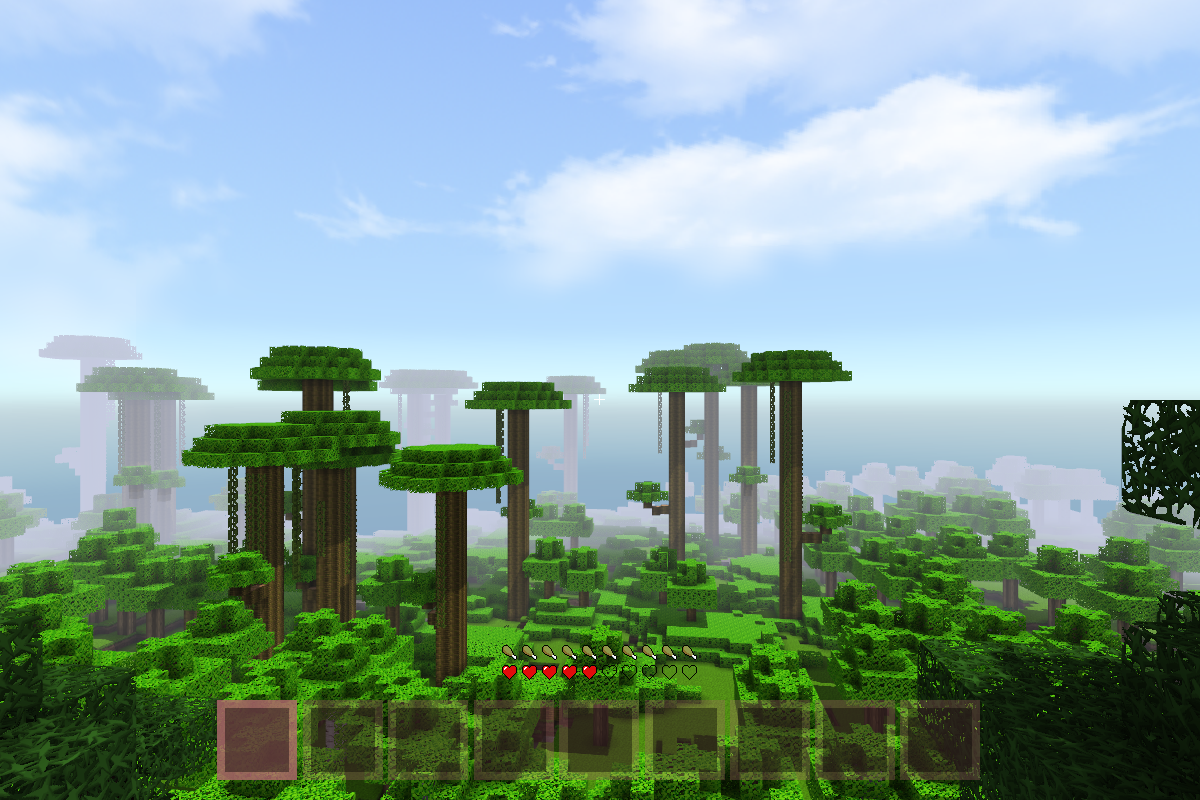
\includegraphics[width=.32\textwidth]{rotate-1.png}
	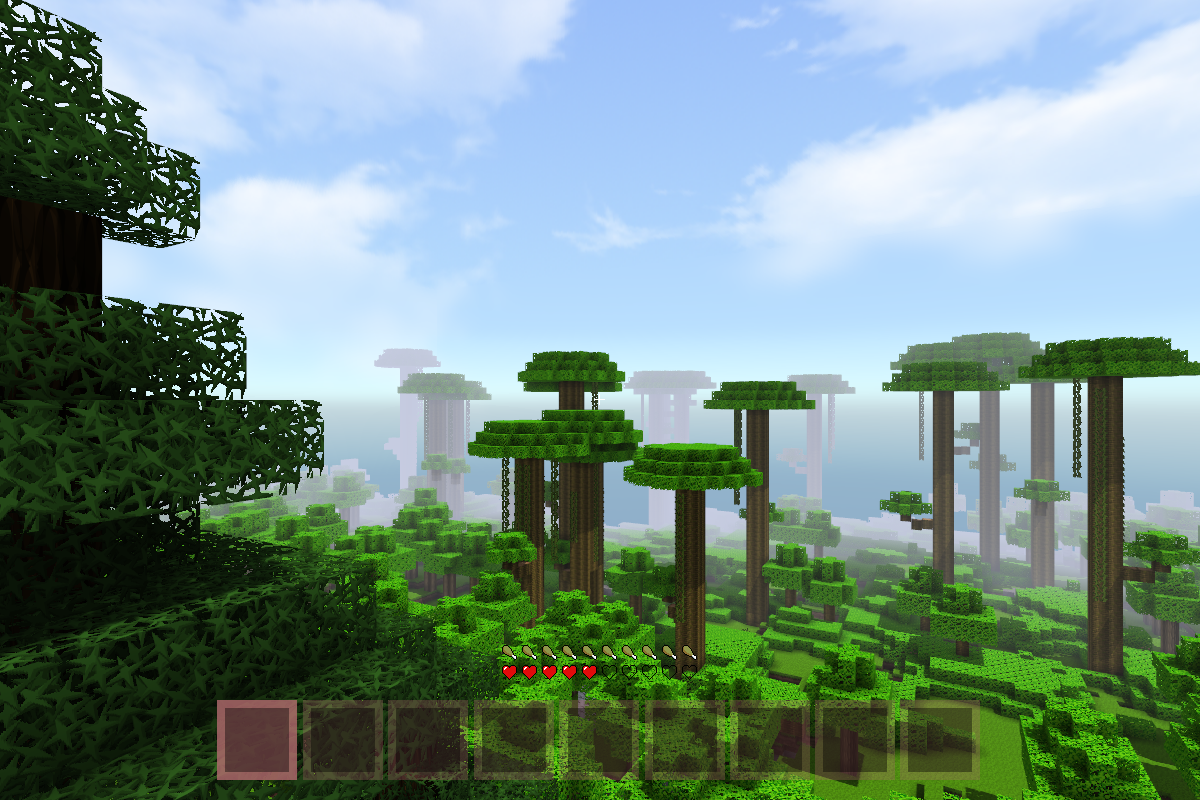
\includegraphics[width=.32\textwidth]{rotate-2.png}
	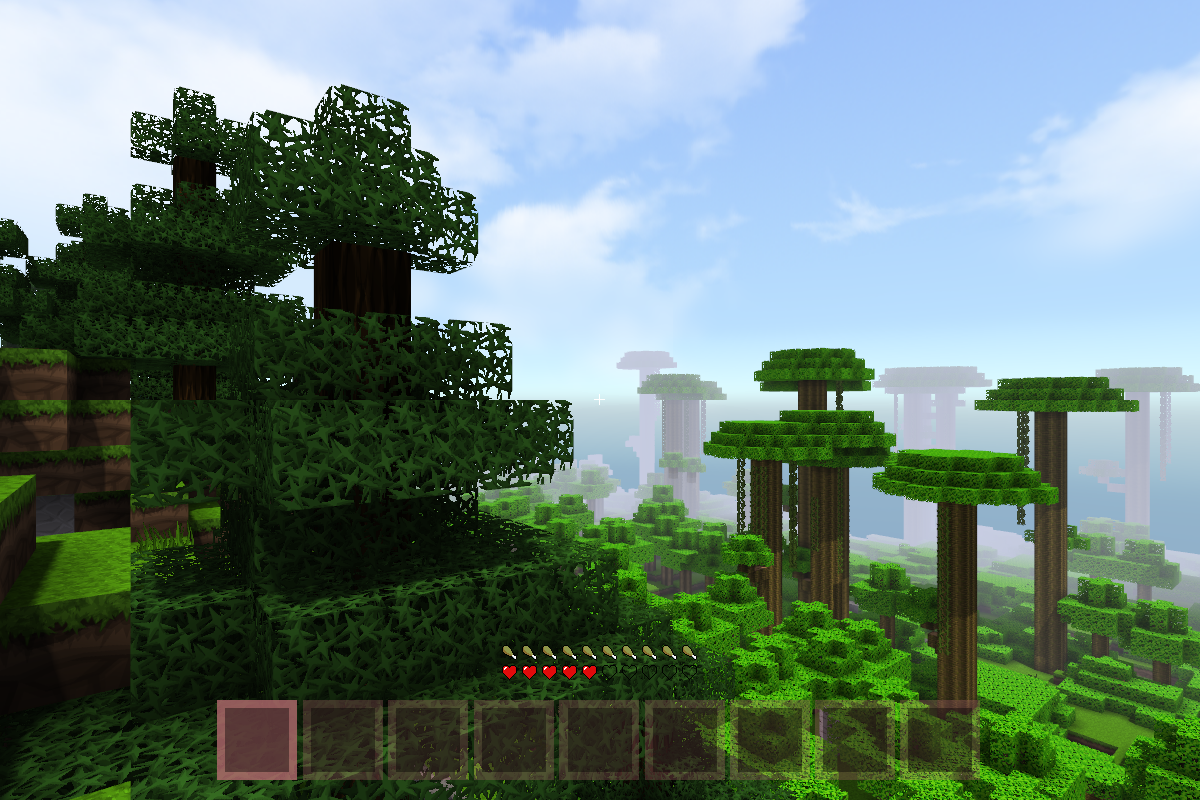
\includegraphics[width=.32\textwidth]{rotate-3.png}\\[4pt]
	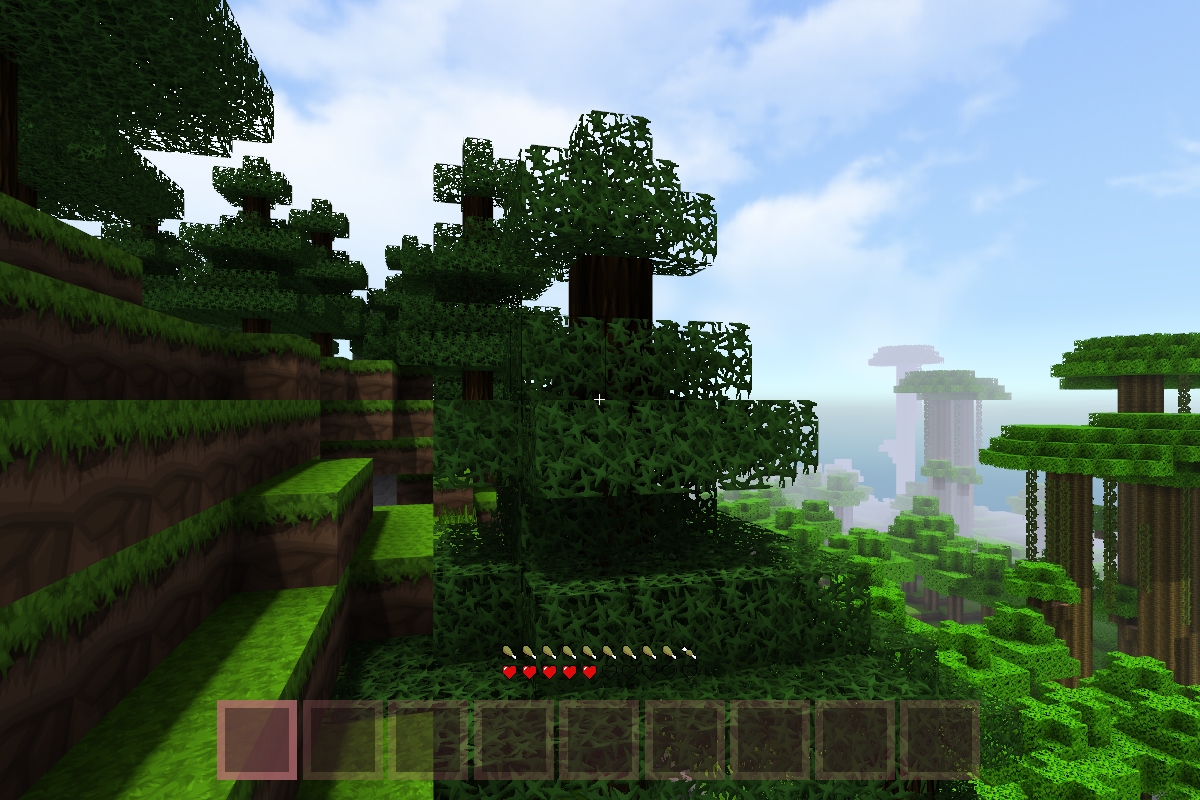
\includegraphics[width=.32\textwidth]{rotate-4.png}
	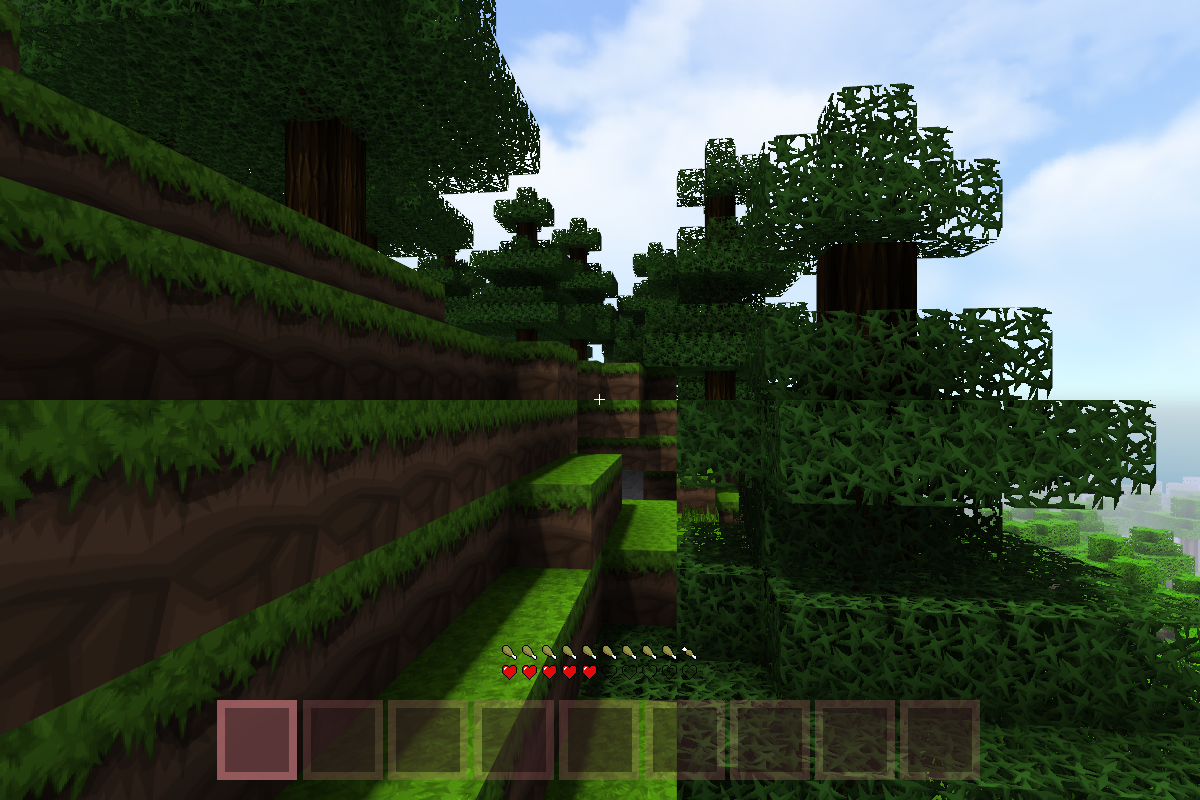
\includegraphics[width=.32\textwidth]{rotate-5.png}
	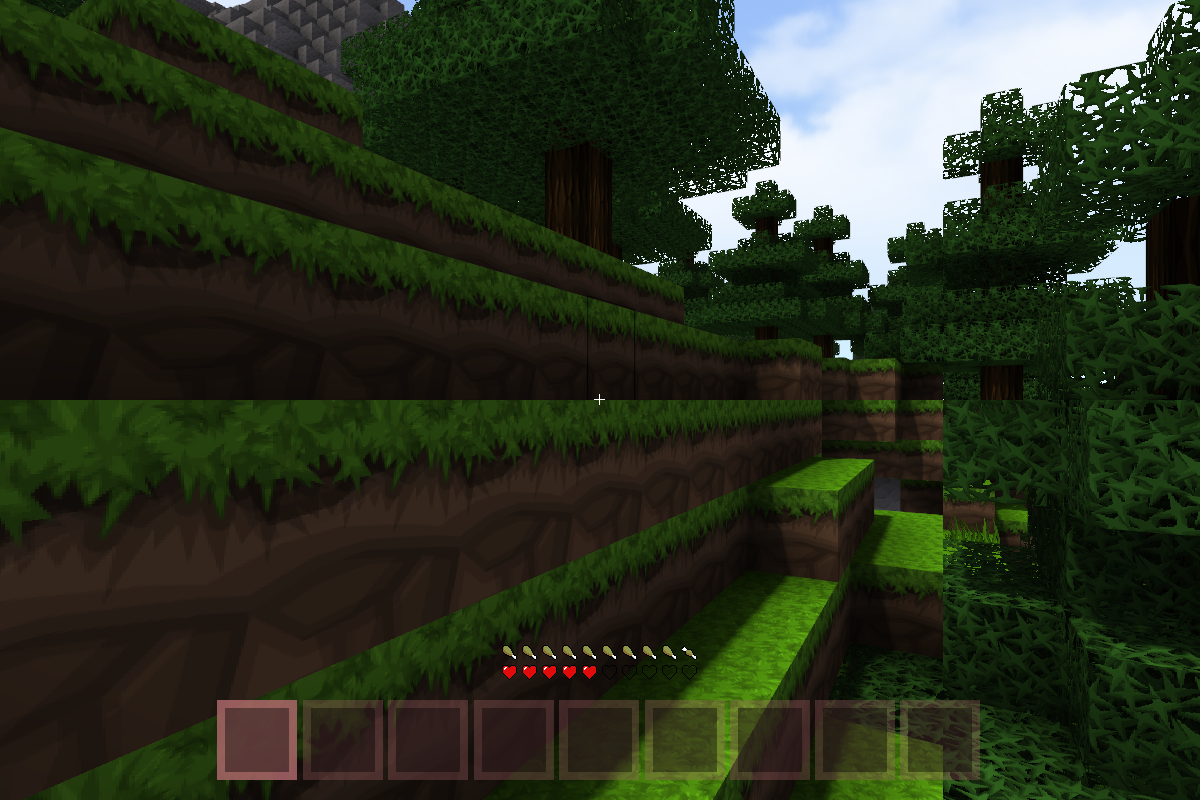
\includegraphics[width=.32\textwidth]{rotate-6.png}
	%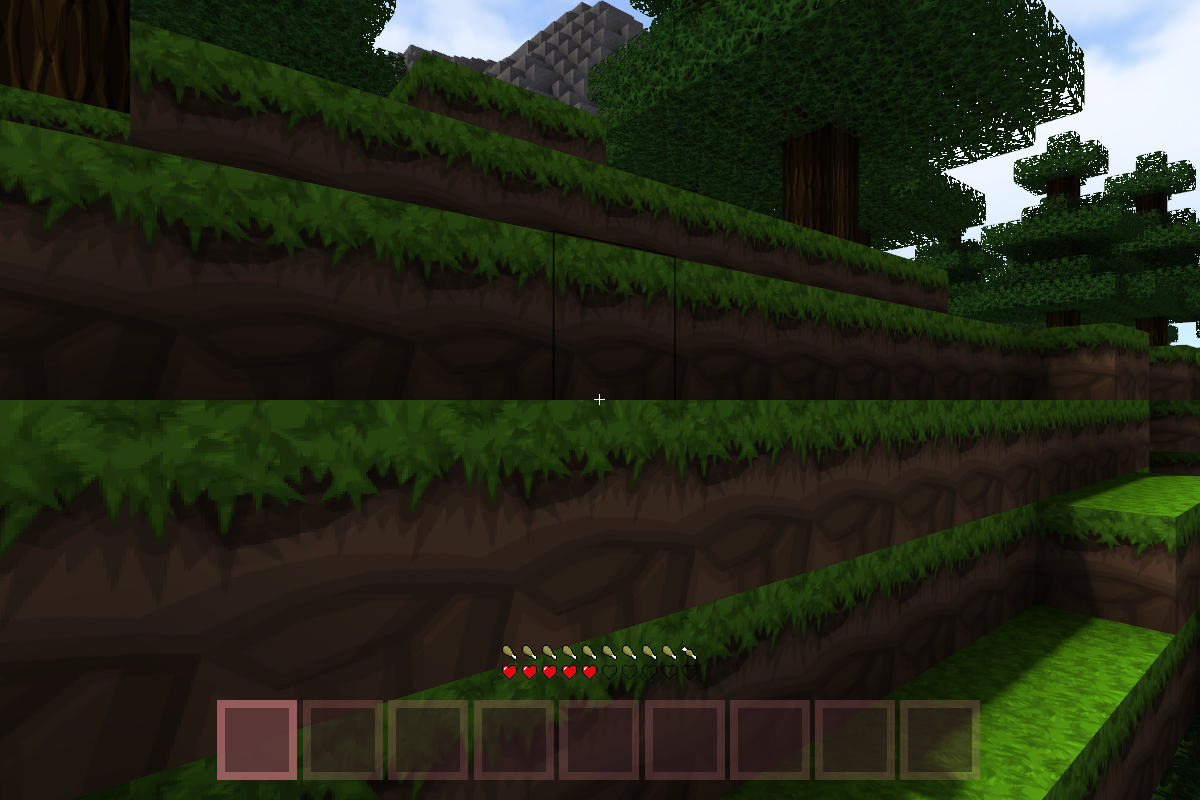
\includegraphics[width=.24\textwidth]{rotate-7.png}
	%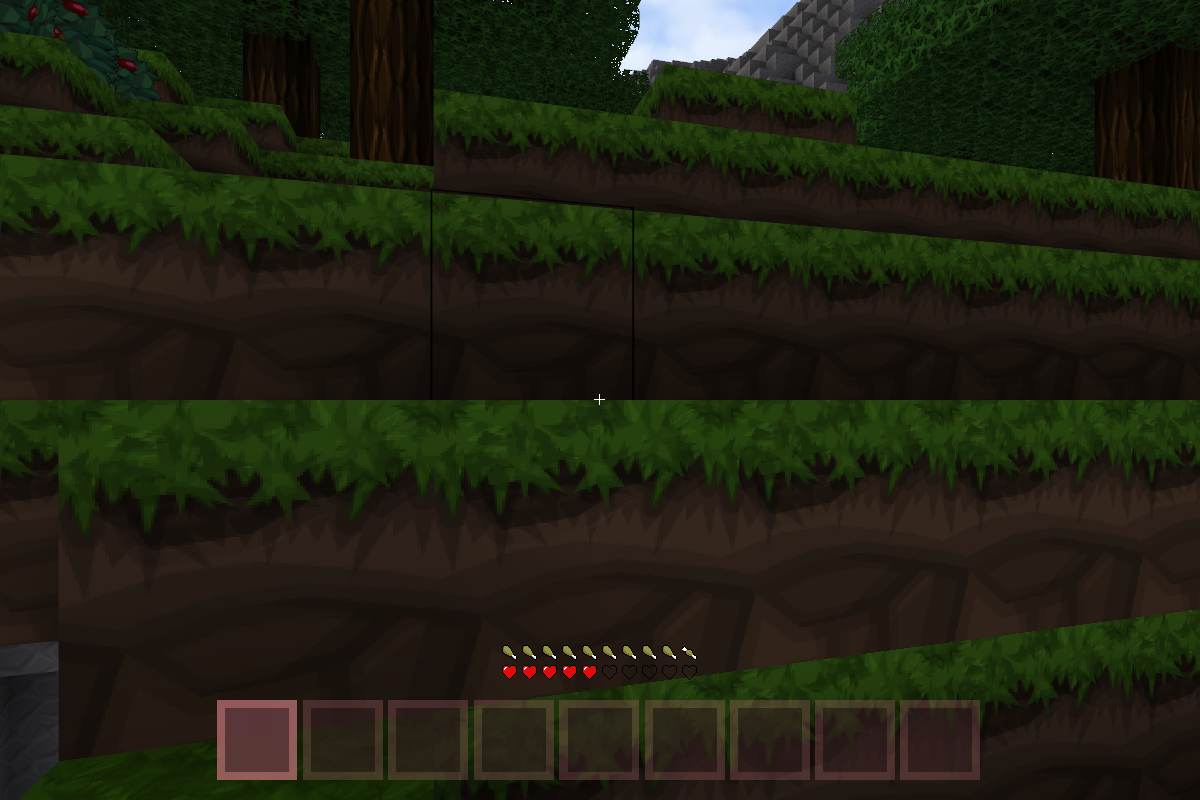
\includegraphics[width=.24\textwidth]{rotate-8.png}
	\caption{Reihe von Screenshots, die die Rotation in Szenario 4 zeigt. Die Rotationsrichtung ist gegen den Uhrzeigersinn. Die Screenshots haben einen Zeitabstand von \SI{500}{\milli\second}.}\label{fig:rotate}
\end{figure}
Wie an den Screenshots zu erkennen ist, wird auch für dieses Szenario der Seed 0 genutzt.

\paragraph{\ac{fps}}
Betrachtet man den Verlauf der \ac{fps} in diesem Szenario ergibt sich ein zu den vorherigen Szenarien sehr verschiedenes Muster. Zu sehen ist das in Abbildung~\vref{fig:seed-0-rotate-fps}.
\begin{figure}[!htbp]
	\fpsplot{seed-0-rotate}
	\caption{Seed 0 Rotation}\label{fig:seed-0-rotate-fps}
\end{figure}
 Zwar ist wieder zu erkennen, dass SystemB ein paar Sekunden später mit der Erzeugung von Bildern beginnt, das Verhalten der Framerate über die Zeit ist danach aber in den Szenarien einzigartig. In SystemA und viel mehr noch in SystemB ist eine zyklische Schwankung der \ac{fps} zu erkennen. Die Periode der Schwankungen beträgt in beiden Systemen \SI{8}{\second}. Das entspricht exakt der Periode der Rotation ($8\cdot45 = 360$). Unter Betrachtung der Screenshots in Abbildung~\vref{fig:rotate} lässt sich eine Hypothese aufstellen, woher diese Schwankungen kommen. In Seed 0 startet der Spielercharakter in der Nähe eines Berges. Ist die Kamera dem Tal zugewandt, müssen deutlich mehr Elemente gezeichnet werden als, wenn die Kamera dem Berg zugewandt ist. Durch die Rotation ändert sich also die Arbeitslast für die \ac{gpu} periodisch.

Durchschnittlich steigt die Bildwiederholrate von \SI{134}{\fps} in SystemA auf \SI{378}{\fps} in SystemB. Das ist eine Steigerung von \SI{182}{\percent}. In beiden System ist die Framerate geringer als im Szenario Welt-Statisch. Der Anstieg der Framerate von SystemA zu SystemB ist allerdings höher. SystemA erreicht ein Maximum von \SI{152}{\fps} und ein Minimum von \SI{113}{\fps}, ein Unterschied von \SI{39}{\fps}. SystemB erreicht maximal \SI{474}{\fps} und singt auf bis zu \SI{287}{\fps}, das ist eine Schwankung von \SI{187}{\fps}.

\paragraph{\ac{cpu}}
Im Gegensatz zu der Bildwiederholrate ist in der Auslastung der \ac{cpu} beinahe keine Schwankung zu erkennen. Insbesondere ist keine Periode von \SI{8}{\second} zu erkennen, wie Abbildung~\vref{fig:seed-0-rotate-cpu} erkennen lässt.
\begin{figure}[!htbp]
	\cpuplot{seed-0-rotate}
	\caption{Seed 0 Rotation}\label{fig:seed-0-rotate-cpu}
\end{figure}
Tatsächlich ist der Graph \ac{cpu}-Auslastung beinahe nicht von dem in Szenario 3 zu unterscheiden, mit der Ausnahme der Startphase. Hier sinkt die Auslastung der \ac{cpu} zum ersten Mal in SystemB zuerst. Die durchschnittliche Auslastung der System ist allerdings identisch zum Welt-Statisch Szenario, \SI{13}{\percent} in SystemA und \SI{23}{\percent} in SystemB.

Die Tatsache, dass die Auslastungsmessung in SystemB zwei Sekunden früher endet, als in SystemA, ist ein Indiz dafür, dass die Messungen aus irgend einem Grund zeitlich verschoben sind. Das würde auch erklären, warum die Startphase in der \ac{cpu}-Auslastung zum ersten Mal in SystemB schneller vorbei ist als in SystemA. Zusätzlich ist die Startphase in der Messung der \ac{fps} in Gegensatz dazu weiterhin mit den vorherigen Szenarien konsistent. 

\paragraph{\ac{gpu}}
Auch der Auslastungsgraph der \ac{gpu} (siehe Abbildung~\vref{fig:seed-0-rotate-gpu}) unterstützt diese Hypothese. Hier ist wieder eine längere Startphase von einigen Sekunden in SystemB zu erkennen. Weiter lässt sich die Aussage scheinbar festigen, dass die Schwankungen der Framerate mit der Auslastung der \ac{gpu} zusammenhängen. Auch hier lässt sich eine achtsekündliche periodische Schwankung erkennen.
\begin{figure}[!htbp]
	\gpuplot{seed-0-rotate}
	\caption{Seed 0 Rotation}\label{fig:seed-0-rotate-gpu}
\end{figure}
Die Tatsache, dass diese Schwankung in SystemA wie bei der Framerate kleiner ist, als in SystemB, führt allerdings zu einer anderen Vermutung. Die Framerate und die \ac{gpu} hängen von der Belastung des Simulations-Threads ab. Die \ac{cpu} des Testsystems besitzt acht Hardware-Threads. Die Auslastung der \ac{cpu} liegt in allen bisherigen Szenarien in SystemA bei \SI{13}{\percent} was in etwa $\frac{1}{8}$ entspricht. Das legt zusammen mit der Tatsache, dass die Auslastung der \ac{gpu} immer unter \SI{100}{\percent} liegt, einen \ac{cpu}-Flaschenhals bezogen auf die Performance nahe. Diese These wird weiter dadurch unterstützt, dass die Verläufe von \ac{fps} und \ac{gpu}-Auslastung deckungsgleich und nicht gegengleich sind. Wäre die höhere Auslastung der \ac{gpu} für eine geringere Bildwiederholrate verantwortlich, müsste das genau anders herum sein.

Diese These ließe sich weiter untersuchen, indem die Auslastung der einzelnen Hardware-Threads gemessen wird. Diese Messung lässt sich in dieser Arbeit leider nicht mehr durchführen. 

Durchschnittlich liegt die Auslastung der \ac{gpu} in SystemA bei \SI{37}{\percent} und in SystemB bei \SI{53}{\percent}. Das ist ein Anstieg von \SI{43}{\percent}.

\paragraph{\ac{ram}}
Die Nutzung des Hauptspeichers, zu sehen in Abbildung~\vref{fig:seed-0-rotate-mem}, ist in Szenario Welt-Rotation grob vergleichbar mit Szenario Welt-Statisch.
\begin{figure}[!htbp]
	\memplot{seed-0-rotate-single-mem.csv}
	\memplot{seed-0-rotate-multi-mem.csv}
	\caption{Seed 0 Rotation}\label{fig:seed-0-rotate-mem}	
\end{figure} 
SystemA nutzt mit durchschnittlich \SI{1267}{\mega\byte} etwas mehr Speicher, SystemB mit \SI{1441}{\mega\byte} aber weniger. Somit ergibt sich in diesem Szenario ein Anstieg von \SI{14}{\percent} statt \SI{44}{\percent}. 

Der selbe Trend lässt sich im kurzweiligen Verbrauch von Speicher erkennen. SystemA hat einen Verbrauch von durchschnittlich \SI{101}{\mega\byte\per\second} und SystemB nutzt \SI{187}{\mega\byte\per\second} was einen Anstieg von \SI{85}{\percent} bedeutet.
